%学会発表レジュメ ver. 1.0

\documentclass[uplatex,twocolumn]{jsarticle}
\usepackage[top=20mm,bottom=20mm,left=20mm,right=20mm]{geometry}
\usepackage[T1]{fontenc}
\usepackage{txfonts}
\usepackage{wrapfig}
\usepackage{multicol}
\usepackage[expert,deluxe]{otf}
\usepackage[dvipdfmx,hiresbb]{graphicx}
\usepackage{here}
\usepackage{epsf}
\usepackage{graphicx}
\usepackage{graphics}
\usepackage{graphicx}

\makeatletter


  \renewcommand{\section}{%
    \if@slide\clearpage\fi
    \@startsection{section}{1}{\z@}%
    {\Cvs \@plus.5\Cdp \@minus.2\Cdp}% 前アキ
    {.5\Cvs \@plus.3\Cdp}% 後アキ
    %{\normalfont\Large\headfont\raggedright}}
    {\normalfont\raggedright}}

  \renewcommand{\subsection}{\@startsection{subsection}{2}{\z@}%
    {\Cvs \@plus.5\Cdp \@minus.2\Cdp}% 前アキ
    {.5\Cvs \@plus.3\Cdp}% 後アキ
    %{\normalfont\large\headfont}}
    {\normalfont}}

  \renewcommand{\subsubsection}{\@startsection{subsubsection}{3}{\z@}%
    {\Cvs \@plus.5\Cdp \@minus.2\Cdp}%
    {\z@}%
    %{\normalfont\normalsize\headfont}}
    {\normalfont}
    } 
    
    
 \newenvironment{figurehere}
    {\def\@captype{figure}}
    {}    
    
\makeatother
%ここから上を編集する必要はない.(figure,を追加)




%footnotemarkで脚注の追加
\title{\vspace{-14mm}GitHub上のソフトウェア開発のためのフロー推薦手法 \footnotemark[0]}
\author{若月 純\footnotemark[2]  矢吹 太朗\\ 千葉工業大学 社会システム科学部 プロジェクトマネジメント学科\footnotemark[3]}
\date{}%日付を入れる必要はない.
\pagestyle{empty}
\begin{document}




\twocolumn[
	\maketitle
]
\begingroup
\def\thefootnote{\fnsymbol{footnote}}
\footnotetext[0]{Workflow recommendation method for software development on GitHub}
\footnotetext[2]{Jun WAKATSUKI(s1242132hb@s.chibakoudai.jp)}
\footnotetext[3]{Department of Project Management, Social System Sciences, Chiba Institute of Tchnology}
\endgroup

\section{序論}

ソフトウェア開発では,複数のメンバが同時に開発を行うため,ファイルの最新バージョンが分からなくなる,同一ファイルに対する変更が競合する等の問題が発生する.このような問題を解決するため,バージョン管理システムを用いる.バージョン管理システムとは,変更履歴を管理するシステムのことである\cite{ikeda2014}.

バージョン管理システムを提供するサービスに,GitHubがある.GitHubは,バージョン管理システムに加え,branch,Pull Requestといった開発を補助する機能を提供するサービスである.branchとは,履歴を分岐して記録していくためのものである.branchを用いることにより,同一リポジトリ内で,別々の作業を並行して行うことが出来るようになる.Pull Requestとは,自分のリポジトリから相手のリポジトリへ,変更を取り込んでもらうための要求を出す機能である.Pull Requestを用いることにより,変更が追加される前に確認することが出来る.

GitHubを使用する手順を開発フローと呼ぶ.開発フローの種類を調査した結果,13種類あることがわかった.開発フローの例として,GitHub フローとGit フローを紹介する.

GitHub フローは,作業をするbranchを作成し,完成したら統合する.といった開発フローである.この開発フローはとてもシンプルなため,開発フローを実施するまでの学習コストは抑えられるが,開発規模が大きい場合,Pull Requestがたまりやすく,コードレビューに時間がかかってしまうことがある.

Git フローは,develop branchから作業用branchを作成する.完成したらPull Requestを行い,作業用branchをdevelop branchに統合する.リリースができるレベルになったら,リリース用branchを作成し,作業をする.リリース作業が終了するとmasterブランチに統合され,バージョンタグを打ってリリースする.といった開発フローである.branch別にやることが決まっているため管理は容易であるが,branchが複数あるため,Pull Requestを異なったbranchに送ってしまう等の人的ミスが発生する場合がある\cite{ohtsuka2014}.

このように,開発フローは,メリットとデメリットがある.しかし,選択する基準は定められていないため,状況にあった開発フローを選択するのは難しい.そのため,適切でない開発フローを選択し,開発に悪影響を与える危険がある.このような事態を防ぐため,適切な開発フローを選択できるようにするための基準が求められる.


そこで本研究では,適切な開発フローを選択できるようにするための基準を求める.
そのために,GitHub上のプロジェクトを対象に,採用されている開発フローと,開発フローの採用に関わると思われる指標を調査し,分析する.

\section{目的}

GitHubを用いたソフトウェア開発プロジェクトの性質において,適切な開発フローを選択できるようにするための基準を求める.

\section{手法}


本研究は3段階に分かれる.
\begin{enumerate}
\item GitHub上のプロジェクトから,開発フローの採用に関わると思われる指標と,採用されている開発フローを調査する.
\item 調査結果を分析する.
\item 分析結果の精度と再現率を求める. 
\end{enumerate}

初めに,GitHub上のプロジェクトから,開発フローの採用に関わると思われる指標を調査する.
本研究で用いた指標は,プロジェクト経過日数,行数,ファイル数,バイト数,Watch数,Star 数,Fork数,Commit数,branch数,Release数,人数,Open Issue数,Closed Issue数,Issue数,Open Pull Request数,Closed Pull Request数,Pull Request数,Label数,Open Milestone数,Closed Milestone数,Milestone数,Wiki数,言語,1日あたりの行数,1日あたりのCommit数,1人日あたりの行数,1人日あたりのCommit数である.

次に,採用されている開発フローを調査する.開発フローの正解データは,人手で作成する.
開発フローは,GitHub上のbranchとPull Requestの特性から求められる.
ここでは,32件のプロジェクトの,5個の開発フロー(Git フローとGitHub フロー,LINE フロー,GitLab フロー,日本CAW フロー)を特定した.
たとえば,develop branchとrelease branchがある場合は,Git フローである.master branchから記述的な名前のbranchがある場合は,GitHub フローである.バージョンごとにbranchが作られている場合は,LINE フローである.branchにstableが用いられている場合は,GitLab フローである.Pull Request にWIPがある場合は,日本CAW フローである.


プロジェクトに関する上述の指標から,開発フローを決めるための決定木の作成を試みる.
具体的には,32件のプロジェクトをランダムに22件の訓練データと10件のテストデータに分け,訓練データを用いて決定木を作成し,テストデータを用いてその性能を測定する.
そのような実験を10回繰り返すことで,精度と再現率の平均と信頼区間を求める.

\section{結果}

% 大文字のHを使用することで好きな位置に図を配置
\begin{figure}[H]
%\includegraphics[width=図の幅,clip]{ファイル名}\label{参照用ラベル}
\includegraphics[width=8.2cm,clip]{decisiontree.eps}
\caption{プロジェクトの性質により選択される開発フローの違い}\label{決定木}
\end{figure}


GitHub上の32件のプロジェクトから,開発フローの採用に関わると思われる指標と,採用されている開発フローを調査し,決定木分析を行った.その結果が,図1である.

図1より,Star数,人数,1日あたりのCommit数,Open Pull Request数,プロジェクト経過日数で,選択されている開発フローを割り出せられる.
たとえば,Star数が129以上かつ,人数が84人未満かつ,Open Pull Requestが1以上かつ,プロジェクト経過日数が707日以上の場合は,Git フローを選択する.


開発フローのわかっているプロジェクトを使って作成された開発フローの決定木が,開発フローが未知のプロジェクトの開発フローを予測できるかどうかを試したところ,精度は平均$41$\%(信頼区間は$26\sim 56$\%),再現率は平均$51$\%(信頼区間は$29\sim 73$\%)だった.


\section{考察}

図1は,全データをStar数で分類している.Starとは,注目度を表す指標である.Star数が129以上の場合,プロジェクトを主にbranchで管理するGit フローが選択されている.Star数が129未満の場合,プロジェクトを主にPull Requestで管理する日本CAW フローが選択されている.ここから,開発人数だけでなく,チェックしているユーザ数により,最適な開発フローが異なることがわかる.

また,1日あたりのCommit数といった,時系列データにより分類されていることが分かった.ここから,Commit増加傾向や,人数の増減傾向等,他の時系列データを調査することで,より精度と再現率をあげられると考えられる.



\section{結論}

本研究では,決定木を用いた,開発フローを推薦する手法を提案した.
現状では,精度と再現率が高いとは言えないが,このような手法を発展させることによって,GitHubの経験が少ないチームでの開発でも,最適なフローを決定できるようになることが期待される.

\bibliographystyle{junsrt}
\bibliography{biblio}%「biblio.bib」というファイルが必要.


\end{document}